%%%%%%   TIPO DE DOCUMENTO: Artículo   %%%%%%
\documentclass[letterpaper,11pt,twoside]{report}

\usepackage[spanish]{babel} %Idioma
\usepackage{graphicx} %Imágenes
\usepackage[utf8]{inputenc} %Acentos
\usepackage{hyperref} %Links
\usepackage{xspace}

\usepackage{listings}
\usepackage{verbatim}
\usepackage{amsmath, amssymb}
\usepackage{amsmath}
\usepackage[active]{srcltx}
\usepackage{amssymb}
\usepackage{amscd}
\usepackage{makeidx}
\usepackage{amsthm}
\usepackage{algpseudocode}
\usepackage{algorithm}
\renewcommand{\baselinestretch}{1}
\setcounter{page}{1}
\setlength{\textheight}{21.6cm}
\setlength{\textwidth}{14cm}
\setlength{\oddsidemargin}{1cm}
\setlength{\evensidemargin}{1cm}
\pagestyle{myheadings}
\thispagestyle{empty}
\markboth{\small{Pr\'actica 2, Jorge Martinez.}}{\small{.}}
\date{}

\begin{document}
	\centerline{\bf Redes de computadoras, \today}
	\centerline{}
	\begin{center}
		\Large{\textsc{Estimaci\'on del temporizador de retransmisi\'on (\textit{RTO, retransmission timeout}) en TCP}}
	\end{center}
	
	\centerline{}
	\centerline{\textbf{Martínez Buenrostro Jorge Rafael}}
	\centerline{}
	
	\centerline{$correo, molap96@gmail.com$}
	
        \centerline{Universidad Aut\'onoma Metropolitana} 
	\centerline{Unidad Iztapalapa, M\'exico}
	
	\bigskip
    %-----------Introduccion  

\section*{Introduccion}

\noindent El protoclo de transmisi\'on (TCP) estima el proceso del RTT para predecir el tiempo de espera (timeout) de la fuente, a fin de ajustar el temporizador de retransmisi\'on. El emisor TCP mide el RTT desde el momento que se env\'ia un segmento hasta recibir el acuse de recibo (ACK) correspondiente
    \section*{Procedimiento}

\subsection*{Identificaci\'on de las trazas de audio}
\noindent Para empezar se descargan las trazas y descomprimirlas utilizando los siguientes comando en la terminal de Linux
\begin{figure}[H]
  \centering
  \begin{lstlisting}[frame=single, breaklines=true, basicstyle=\footnotesize\ttfamily, breakatwhitespace=false, 
      columns=flexible, tabsize=2, showstringspaces=false, language=bash] 
    
    wget http://victor.ramos.online.fr/practica1/traces/1.txt.gz
    
    gzip -dk 1.txt.gz

  \end{lstlisting}
  \caption{Comando para descargas y descomprimir las trazas}
  \label{fig:commandDownloadExtract}
\end{figure}

\noindent Para poder caracterizar el retardo de extremo a extremo, la Profra. Sue Moon propone añadir un elemento más a la
diferencia; dicho elemento es la mínima diferencia de retardo encontrada en toda la traza. Esto significa encontrar
\( t_{min}=min\{ t^r_i\}-t^t_i, \forall i\). Como las estampas de tiempo est\'an codificadas con el protocolo RTP y han sido
obtenidas con voz muestreada a 8,000 Hz, finalmente podremos observar el comportamiento del retardo de extremo a extremo
dentro del paquete \textit{i} con:
\begin{equation}
  d^i_{end-to-end}=\frac{t^r_i-t^t_i-t_{min}}{8000}[seg.]
\end{equation}

\noindent Para encontrar el \textit{tiempo de sesi\'on} para cada paquete, el an\'alisis es id\'entico al de una llamada
telef\'onica tradicional, el que llama paga. Entonces, el tiempo de sesi\'on estar\'a basado en el reloj del transmisor. Este
tiempo comenzar\'a a correr a partir de la primera estampara de tiempo \( t^t_i \) hasta la \'ultima \( t^t_N \) dado que
\textit{N} es el n\'umero total de paquetes en la sesi\'on. Entonces:
\begin{equation}
  t^i_{session}=\frac{t^t_i-t^t_i}{8000}[seg]
\end{equation}

\noindent Para analizar el retardo de extremo a extremo, entonces, se realizar\'an las gr\'aficas de las Ecuaciones (1) y (2)
para cada una de las seis trazas, a gran escala y a pequeña escala. La ecuaci\'on (1) es para el eje de las \textit{y} y (2)
para el eje de las \textit{x}.

\subsection*{Manipulaci\'on de trazas con AWK}
\noindent Para analizar algunas estad\'isticas b\'asicas de las sesiones de VoIP capturadas en las trazas, se relizaron los
siguientes scripts en AWK:
\begin{enumerate}
  \item Script para contar el n\'umero total de frases (\textit{talkspurts}) en una traza de retardo.
  \begin{figure}[H]
    \centering
    \begin{lstlisting}[frame=single, breaklines=true, basicstyle=\footnotesize\ttfamily, breakatwhitespace=false, 
        columns=flexible, tabsize=2, showstringspaces=false, language=AWK] 
      
    \end{lstlisting}
    \label{fig:scriptTalksprut}
  \end{figure}

  \item Script para contar el n\'umero total de paquetes que llegaron al receptor.
  \begin{figure}[H]
    \centering
    \begin{lstlisting}[frame=single, breaklines=true, basicstyle=\footnotesize\ttfamily, breakatwhitespace=false, 
        columns=flexible, tabsize=2, showstringspaces=false, language=AWK] 
  
    \end{lstlisting}
    \label{fig:scriptPaquetesRecibidos}
  \end{figure}

  \item Script para encontrar la diferencia m\'inima entre la estampa de tiempo de receptor menos de la del emisor
  \begin{figure}[H]
    \centering
    \begin{lstlisting}[frame=single, breaklines=true, basicstyle=\footnotesize\ttfamily, breakatwhitespace=false, 
        columns=flexible, tabsize=2, showstringspaces=false, language=AWK] 
  
    \end{lstlisting}
    \label{fig:scriptDiferencia}
  \end{figure}

  \item Script que recibe una traza como entrada y entrega en un archivo dos columnas: tiempo de la sesi\'on en segundos, 
  y retardo de extremo a extremo a extremo en segundo.
  \begin{figure}[H]
    \centering
    \begin{lstlisting}[frame=single, breaklines=true, basicstyle=\footnotesize\ttfamily, breakatwhitespace=false, 
        columns=flexible, tabsize=2, showstringspaces=false, language=AWK] 
  
    \end{lstlisting}
    \label{fig:scriptTiempoSesionRetardoExtremoExtremo}
  \end{figure}

  \item Script que calula el retardo promedio de extremo a extremo en una sesi\'on
  \begin{figure}[H]
    \centering
    \begin{lstlisting}[frame=single, breaklines=true, basicstyle=\footnotesize\ttfamily, breakatwhitespace=false, 
        columns=flexible, tabsize=2, showstringspaces=false, language=AWK] 
  
    \end{lstlisting}
    \label{fig:scriptRetardoExtremoExtremoSesion}
  \end{figure}
\end{enumerate}
		%-----------Entregables  
\newpage
\section*{Entregables}

\subsection*{Cálculo del Error Cuadrático Medio (ECM)}
\noindent El error cuadr\'atico medio es una m\'etrica com\'unmente utilizada para evaluar la 
diferencia entre valores predichos y valores reales. La f\'ormula del error cuadr\'atico es:

$$ ECM = \frac{1}{N} \sum_{i = 1}^{N}(x_i-\hat{x}_i)^2 $$

donde 

\begin{itemize}
  \item N es el número total de muestras
  \item \(x_i\) es el valor real de \textit{sampleRTT} en la i-\'esima medici\'on
  \item \(\hat{x}_i\) es el valor estimado de \textit{estimatedRTT} en la i-\'esima medici\'on
\end{itemize}

\noindent Este valor se utiliza para comparar los diferentes valores de \( \alpha \) en el proceso de estimación.

\subsection*{Implementación de la Estimación de RTT}
\noindent Para este análisis, se emplea el algoritmo de Jacobson para estimar el \( \text{EstimatedRTT} \) 
y el \( \text{RTO} \) a partir de las muestras de \( \text{SampleRTT} \). Se emplean tres valores 
diferentes de \( \alpha \) para estudiar su influencia en el cálculo del \( \text{EstimatedRTT} \),
a saber:
\begin{itemize}
    \item \( \alpha = \frac{1}{8} \) (valor por defecto)
    \item \( \alpha_1 = \frac{1}{4} \)
    \item \( \alpha_2 = \frac{1}{16} \)
\end{itemize}

\subsection*{Análisis de Resultados}
\noindent Se realizaron tres simulaciones para cada valor de \( \alpha \), y se calcularon los valores 
de \( \text{SampleRTT} \), \( \text{EstimatedRTT} \) y \( \text{RTO} \) para cada medición. A 
continuación, se presenta el error cuadrático medio (ECM) para cada uno de los valores de \( \alpha \)

\begin{equation}
  \text{MSE}(\alpha) = \frac{1}{n} \sum_{i=1}^{n} ( \text{SampleRTT}_i - \text{EstimatedRTT}_i )^2
\end{equation}

\subsection*{Gráficas de la Estimación de RTT}
\noindent A continuación se presentan las gráficas de los tres procesos: \( \text{SampleRTT} \), 
\( \text{EstimatedRTT} \) y \( \text{TimeoutInterval} \), para cada valor de \( \alpha \) 
seleccionado. El eje \( x \) representa el número de la medición (número de vuelta), 
mientras que el eje \( y \) muestra los valores de los procesos.

\begin{figure}[H]
    \centering
    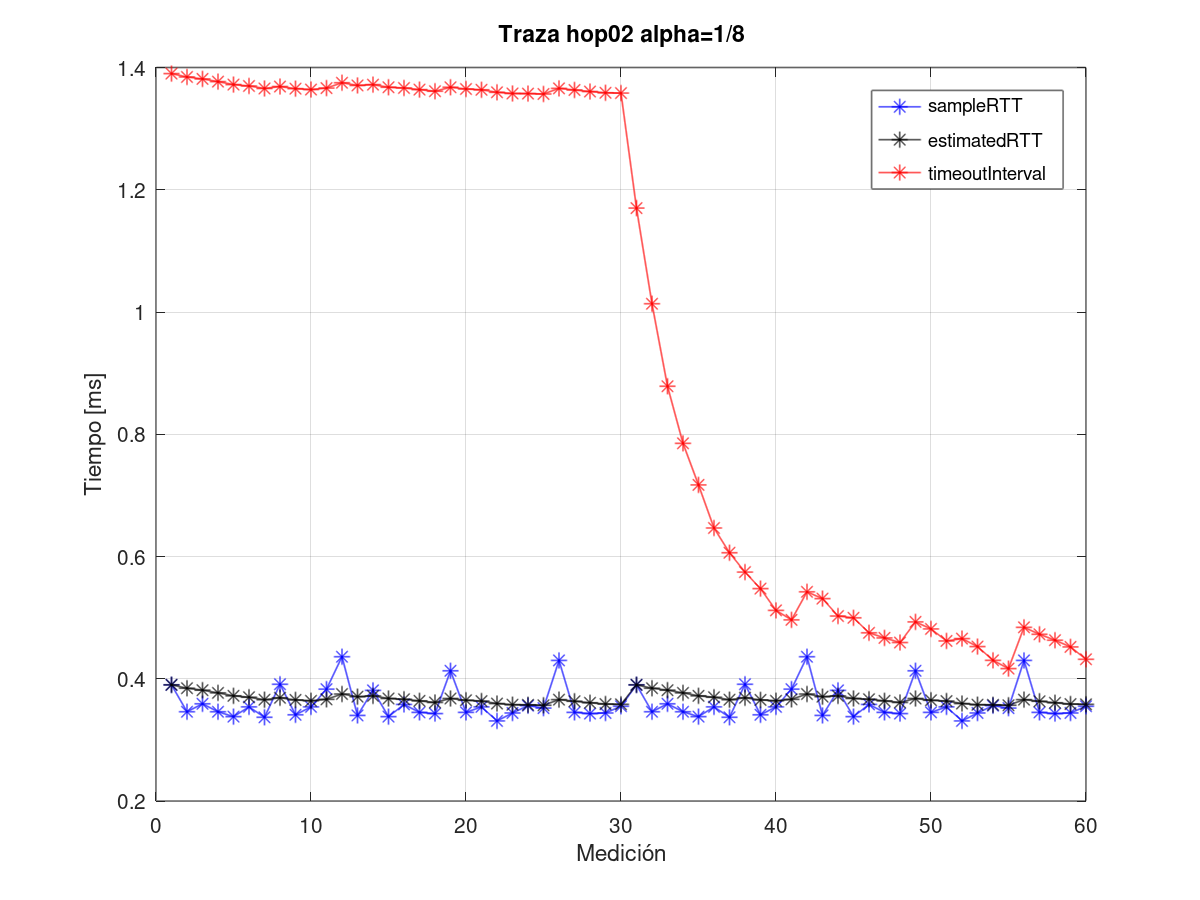
\includegraphics[width=0.75\textwidth]{img/alpha18/trazahop02.png}
    \caption{Gráfica de SampleRTT, EstimatedRTT y TimeoutInterval con \( \alpha = \frac{1}{8} \)
    de la muestra hop02}

    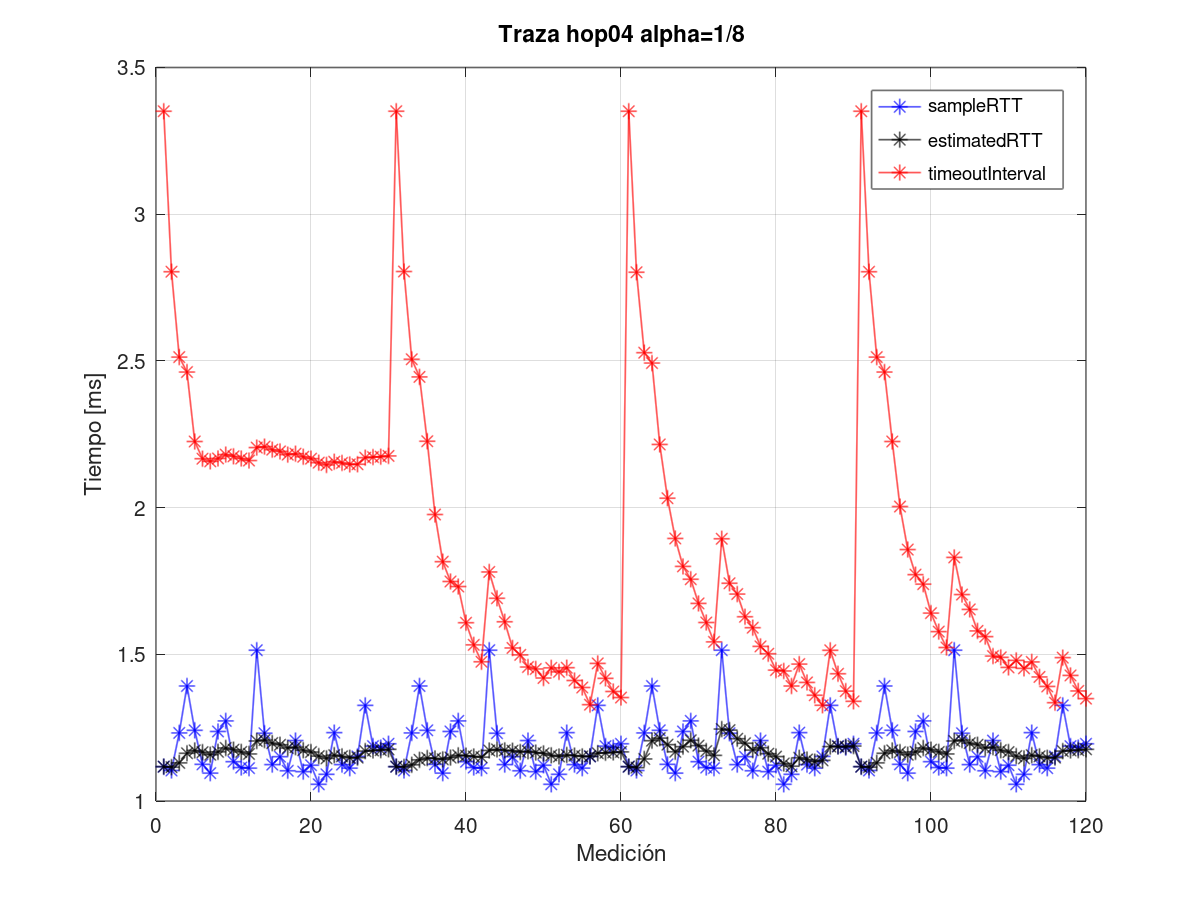
\includegraphics[width=0.75\textwidth]{img/alpha18/trazaHop04.png}
    \caption{Gráfica de SampleRTT, EstimatedRTT y TimeoutInterval con \( \alpha = \frac{1}{8} \)
    de la muestra hop04}
    \label{fig:alpha_default_p1}
\end{figure}
\newpage
\begin{figure}[H]
  \centering
  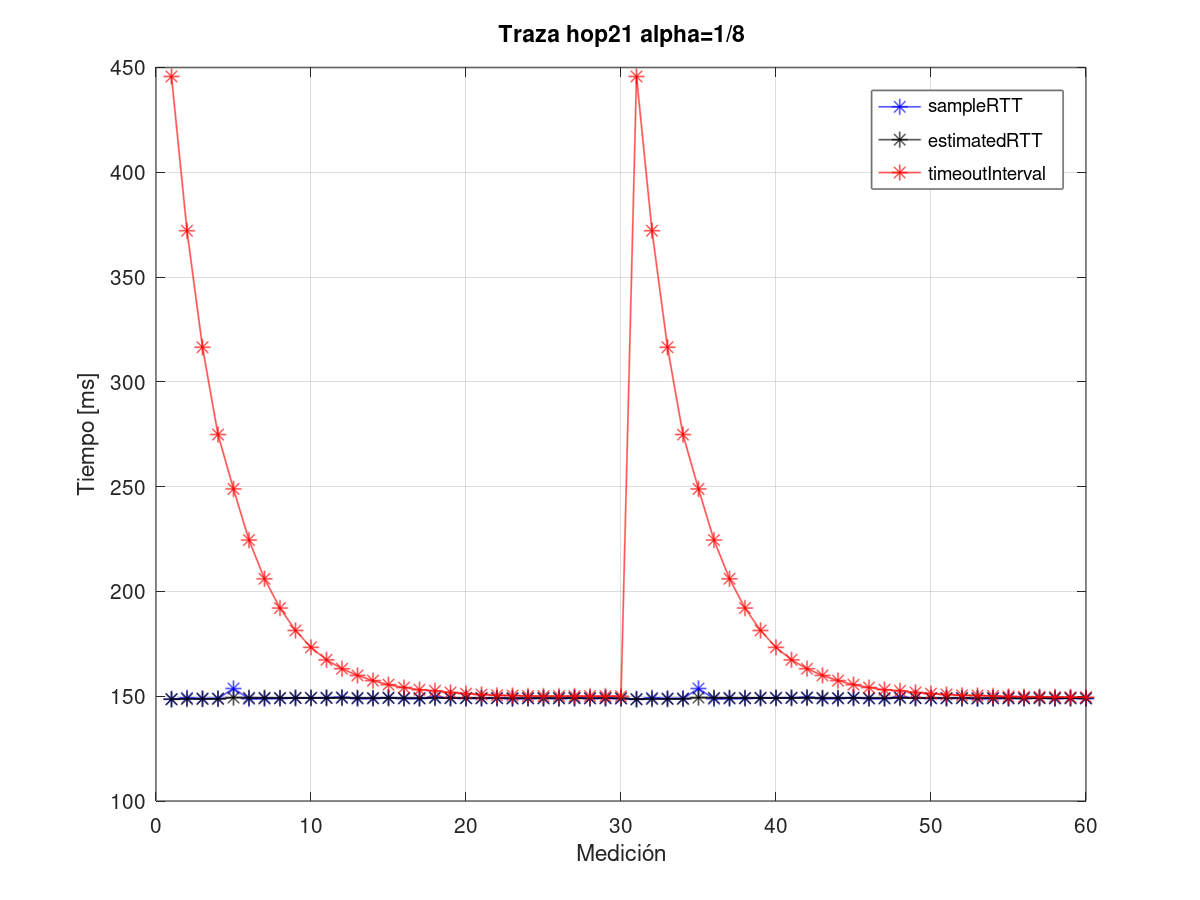
\includegraphics[width=0.75\textwidth]{img/alpha18/trazaHop21.png}
  \caption{Gráfica de SampleRTT, EstimatedRTT y TimeoutInterval con \( \alpha = \frac{1}{8} \)
  de la muestra hop21}

  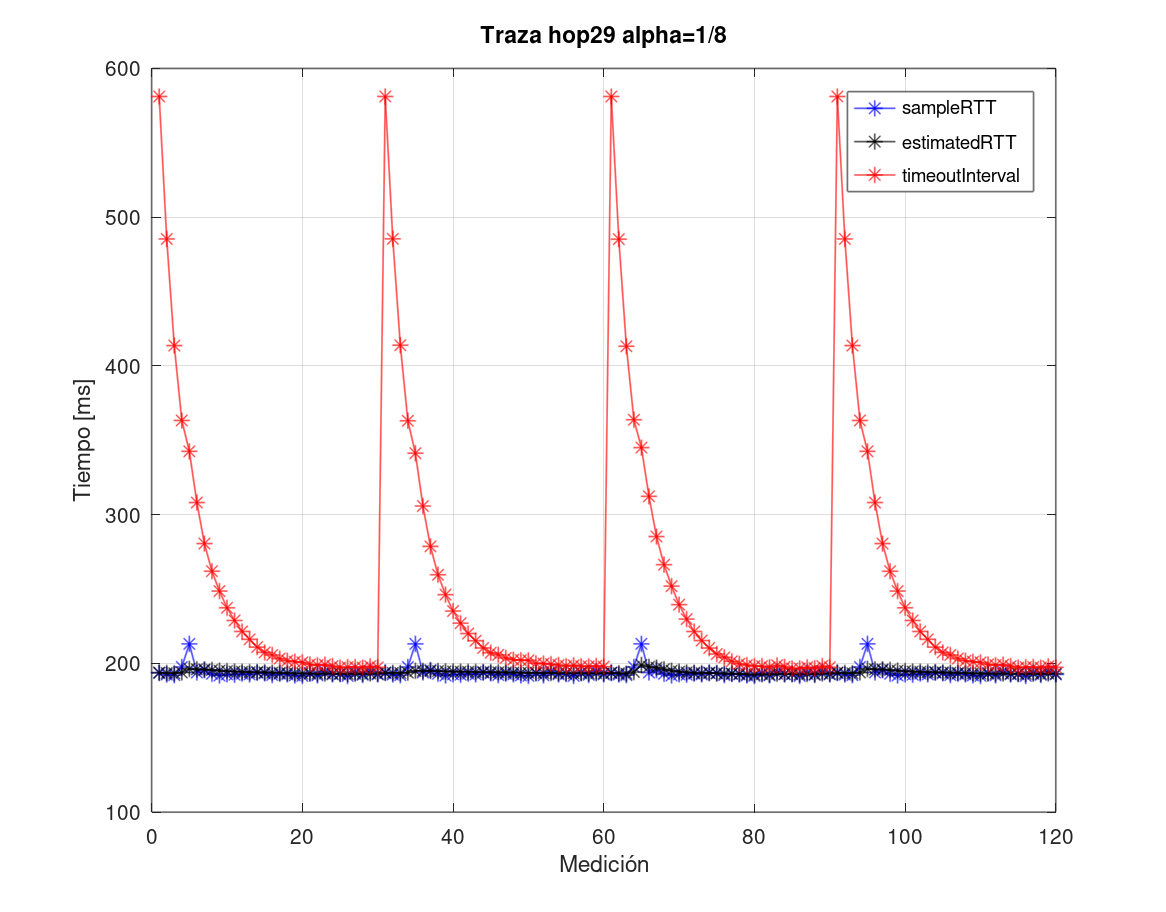
\includegraphics[width=0.75\textwidth]{img/alpha18/trazaHop29.png}
  \caption{Gráfica de SampleRTT, EstimatedRTT y TimeoutInterval con \( \alpha = \frac{1}{8} \)
  de la muestra hop29}
  \label{fig:alpha_default_p2}
\end{figure}

\begin{figure}[H]
    \centering
    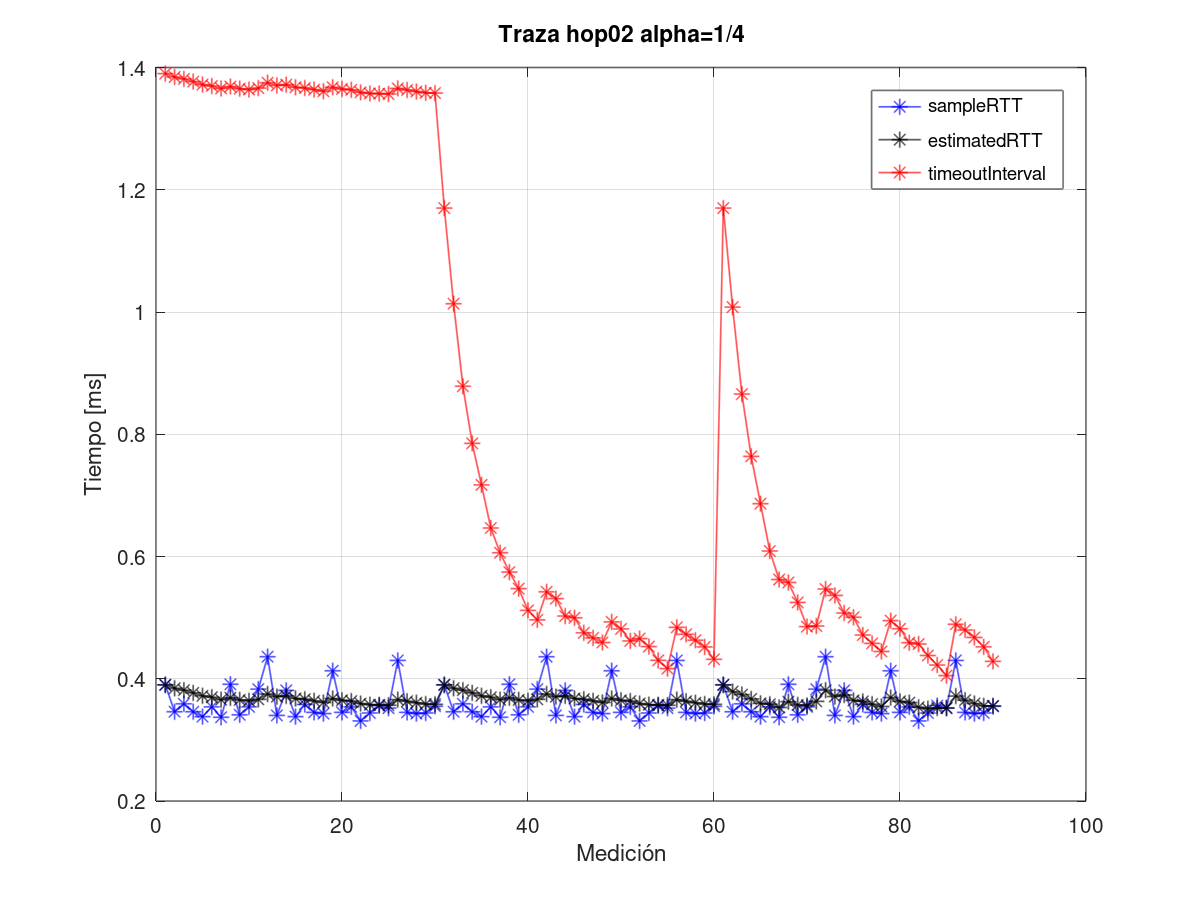
\includegraphics[width=0.75\textwidth]{img/alpha14/trazaHop02.png}
    \caption{Gráfica de SampleRTT, EstimatedRTT y TimeoutInterval con \( \alpha = \frac{1}{4} \)
    de la muestra hop02}

    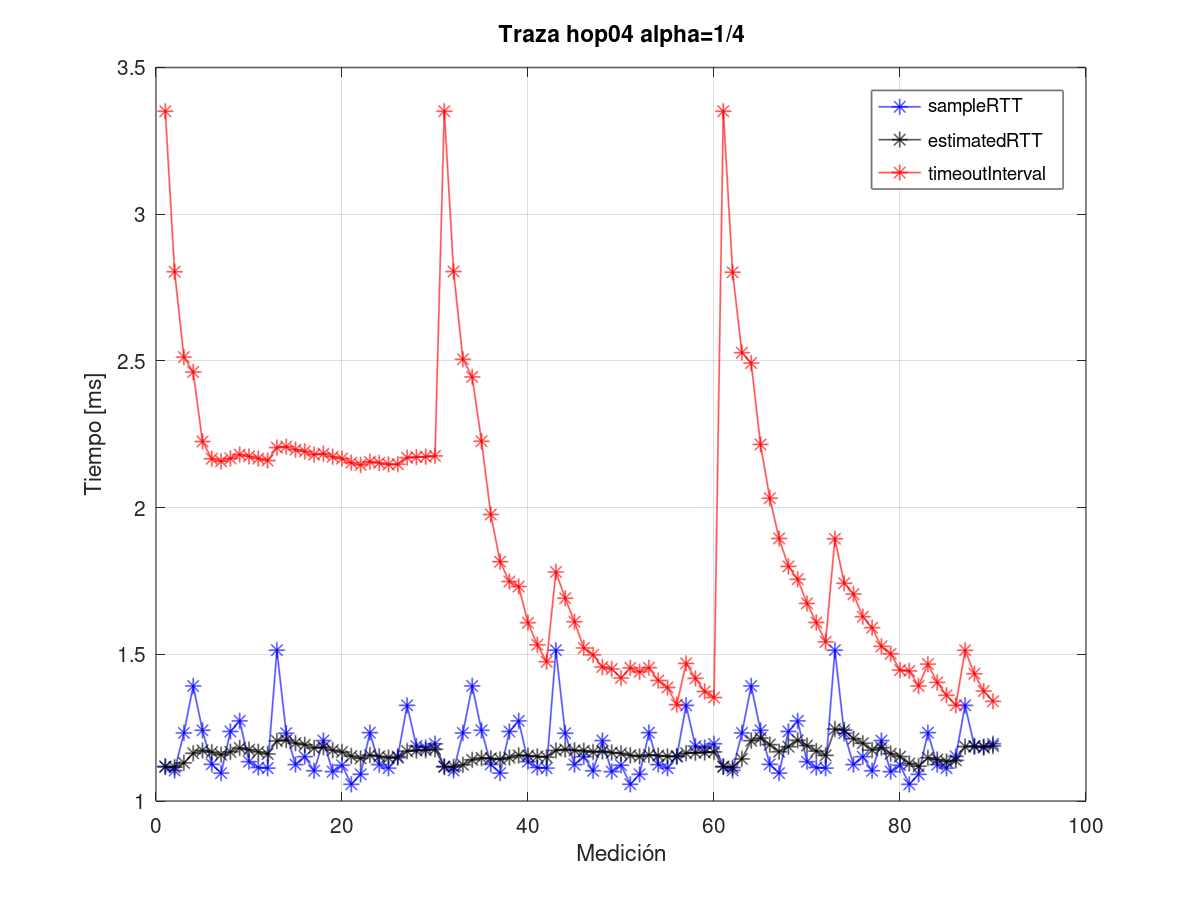
\includegraphics[width=0.75\textwidth]{img/alpha14/trazaHop04.png}
    \caption{Gráfica de SampleRTT, EstimatedRTT y TimeoutInterval con \( \alpha = \frac{1}{4} \)
    de la muestra hop04}
    \label{fig:alpha1_p1}
\end{figure}
\newpage
\begin{figure}[H]
  \centering
  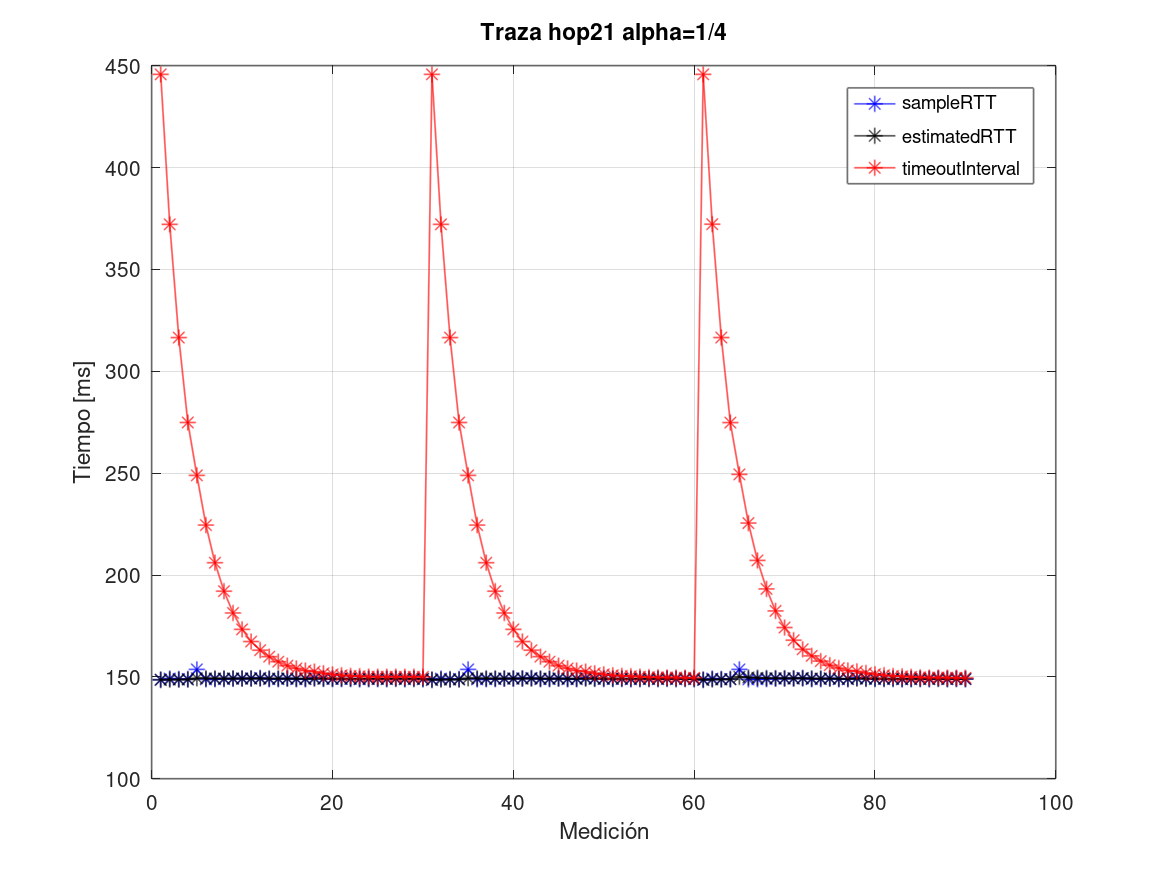
\includegraphics[width=0.75\textwidth]{img/alpha14/trazaHop21.png}
  \caption{Gráfica de SampleRTT, EstimatedRTT y TimeoutInterval con \( \alpha = \frac{1}{4} \)
  de la muestra hop21}

  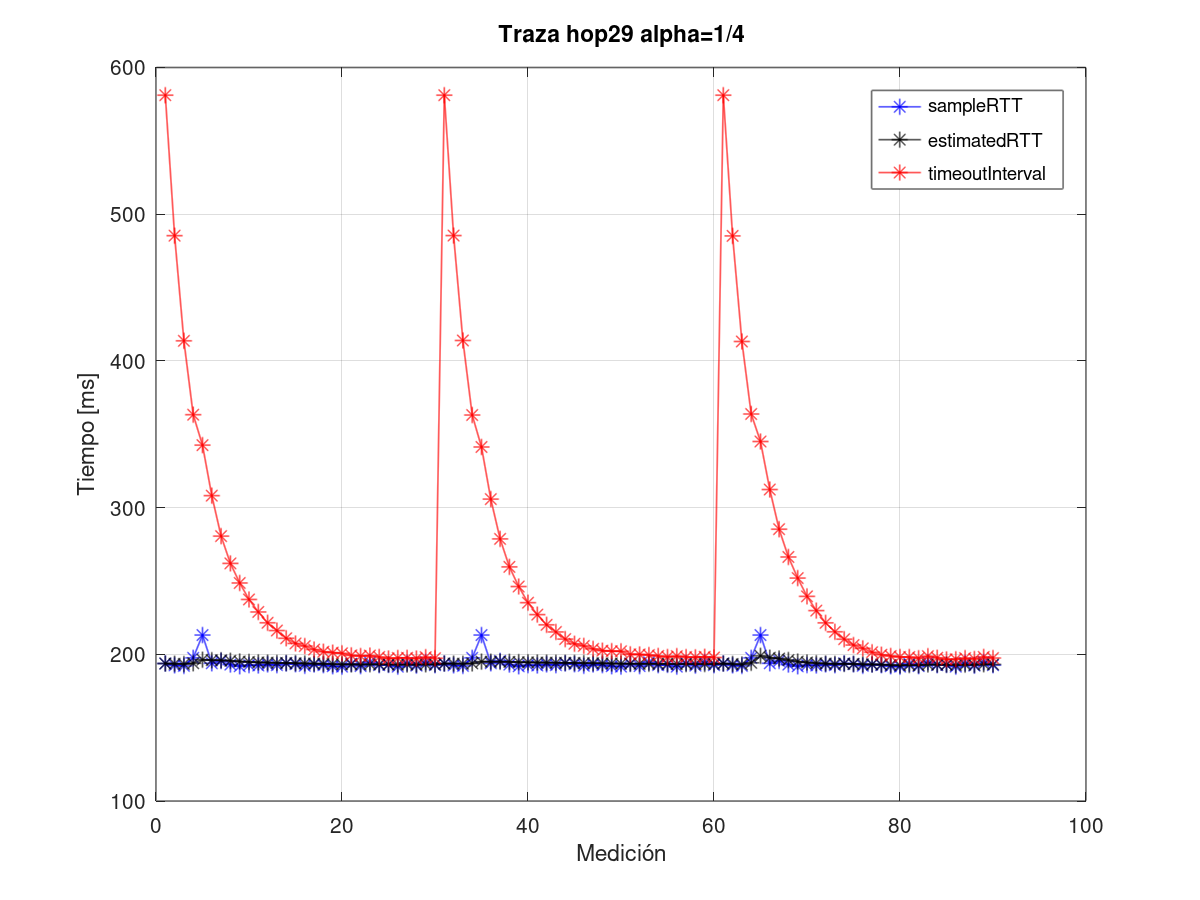
\includegraphics[width=0.75\textwidth]{img/alpha14/trazaHop29.png}
  \caption{Gráfica de SampleRTT, EstimatedRTT y TimeoutInterval con \( \alpha = \frac{1}{4} \)
  de la muestra hop29}
  \label{fig:alpha1_p2}
\end{figure}

\begin{figure}[H]
    \centering
    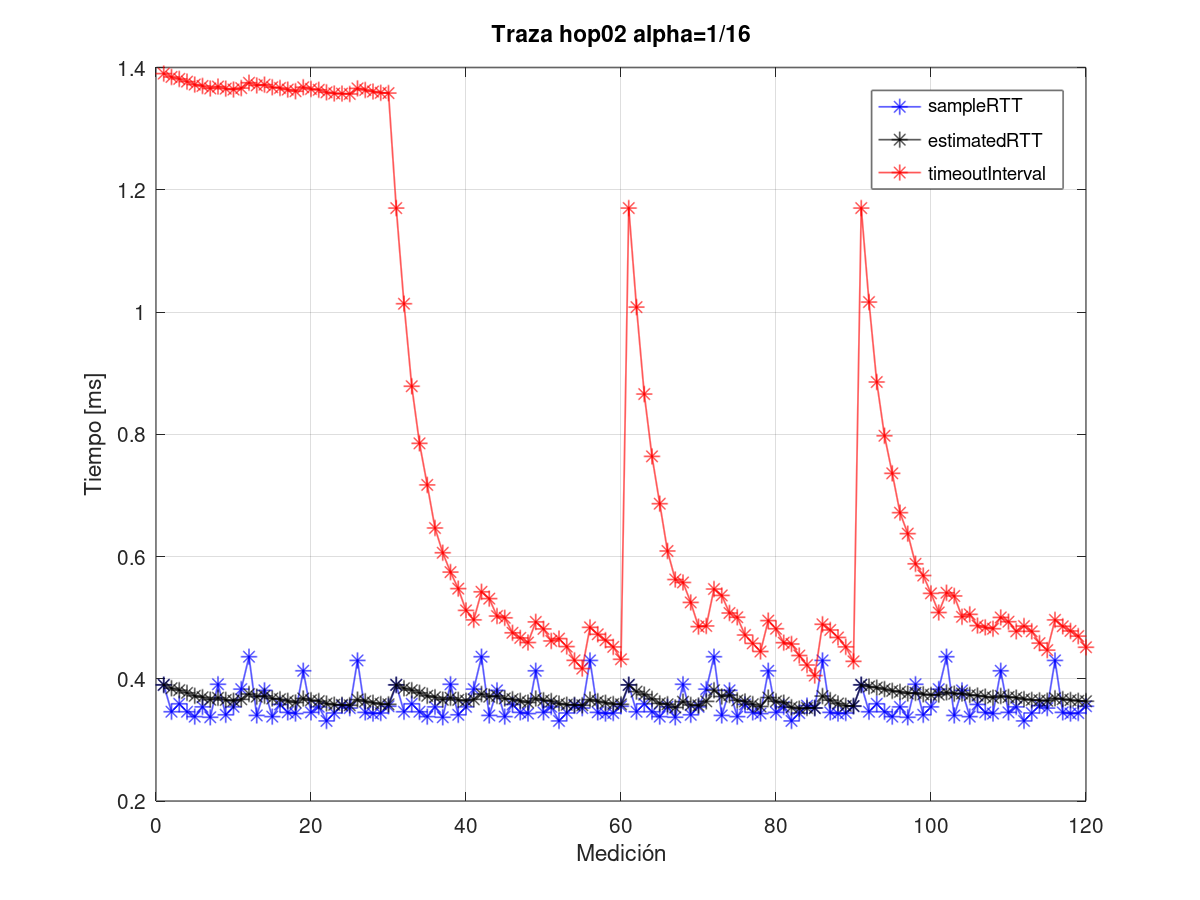
\includegraphics[width=0.75\textwidth]{img/alpha116/trazaHop02.png} 
    \caption{Gráfica de SampleRTT, EstimatedRTT y TimeoutInterval con \( \alpha = \frac{1}{16} \)
    de la muestra hop02}

    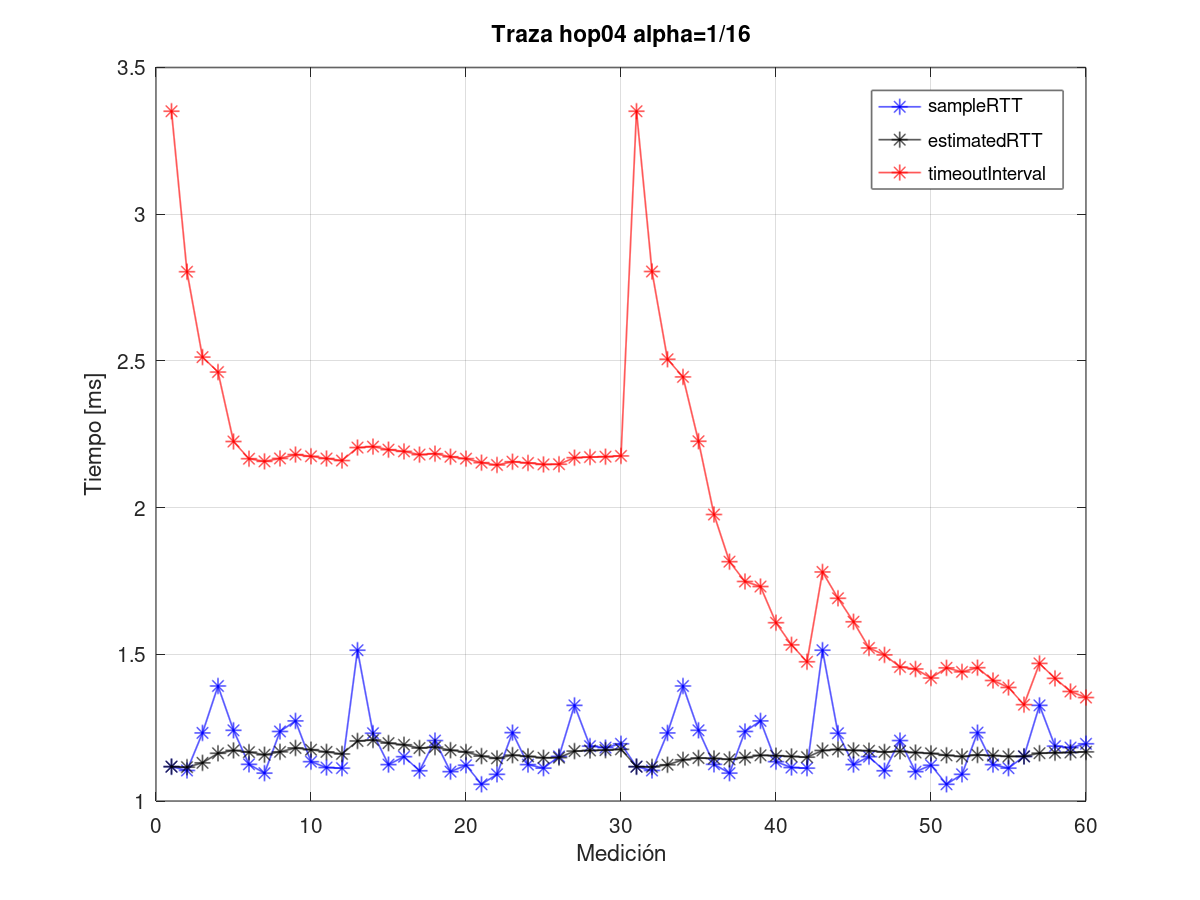
\includegraphics[width=0.75\textwidth]{img/alpha116/trazaHop04.png} 
    \caption{Gráfica de SampleRTT, EstimatedRTT y TimeoutInterval con \( \alpha = \frac{1}{16} \)
    de la muestra hop04}
    \label{fig:alpha2_p1}
\end{figure}
\newpage
\begin{figure}[H]
  \centering
  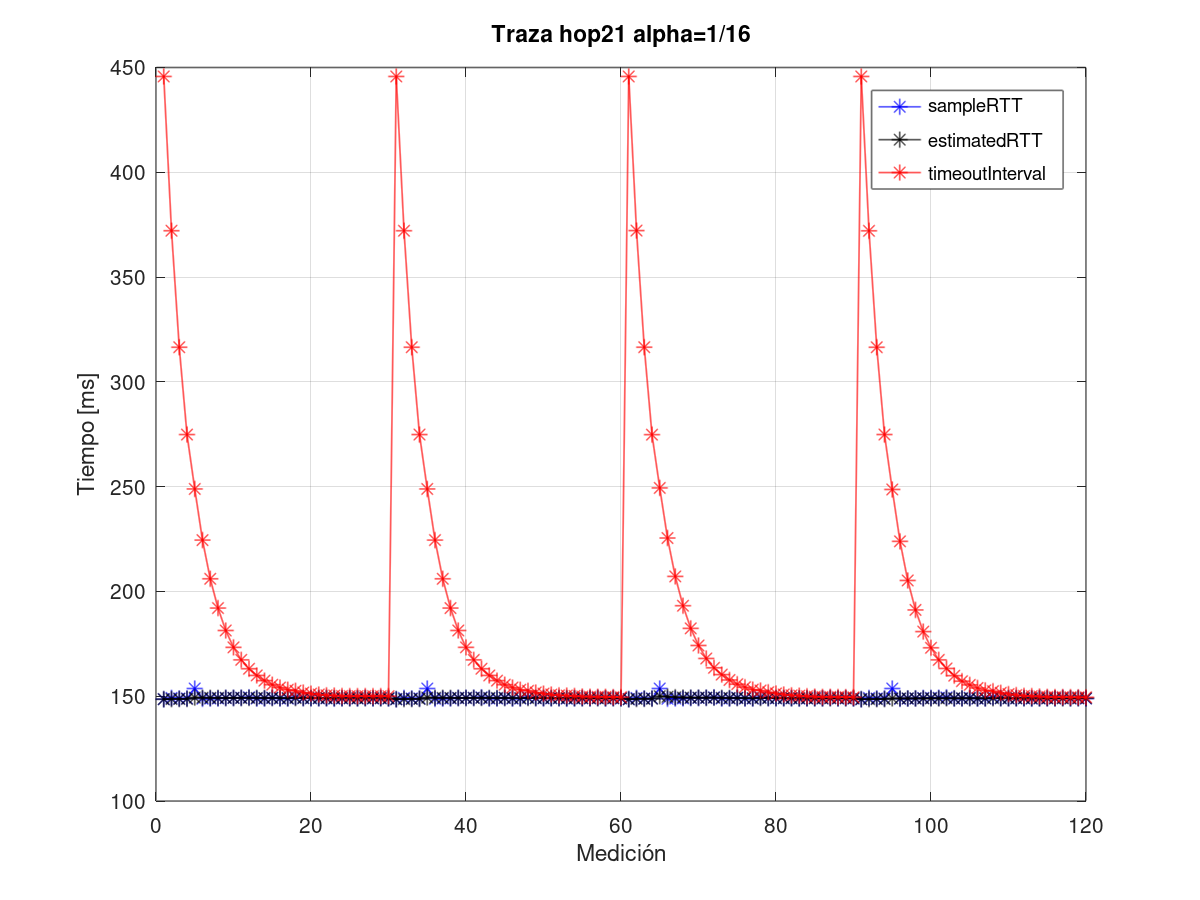
\includegraphics[width=0.75\textwidth]{img/alpha116/trazaHop21.png} 
  \caption{Gráfica de SampleRTT, EstimatedRTT y TimeoutInterval con \( \alpha = \frac{1}{16} \)
  de la muestra hop21}

  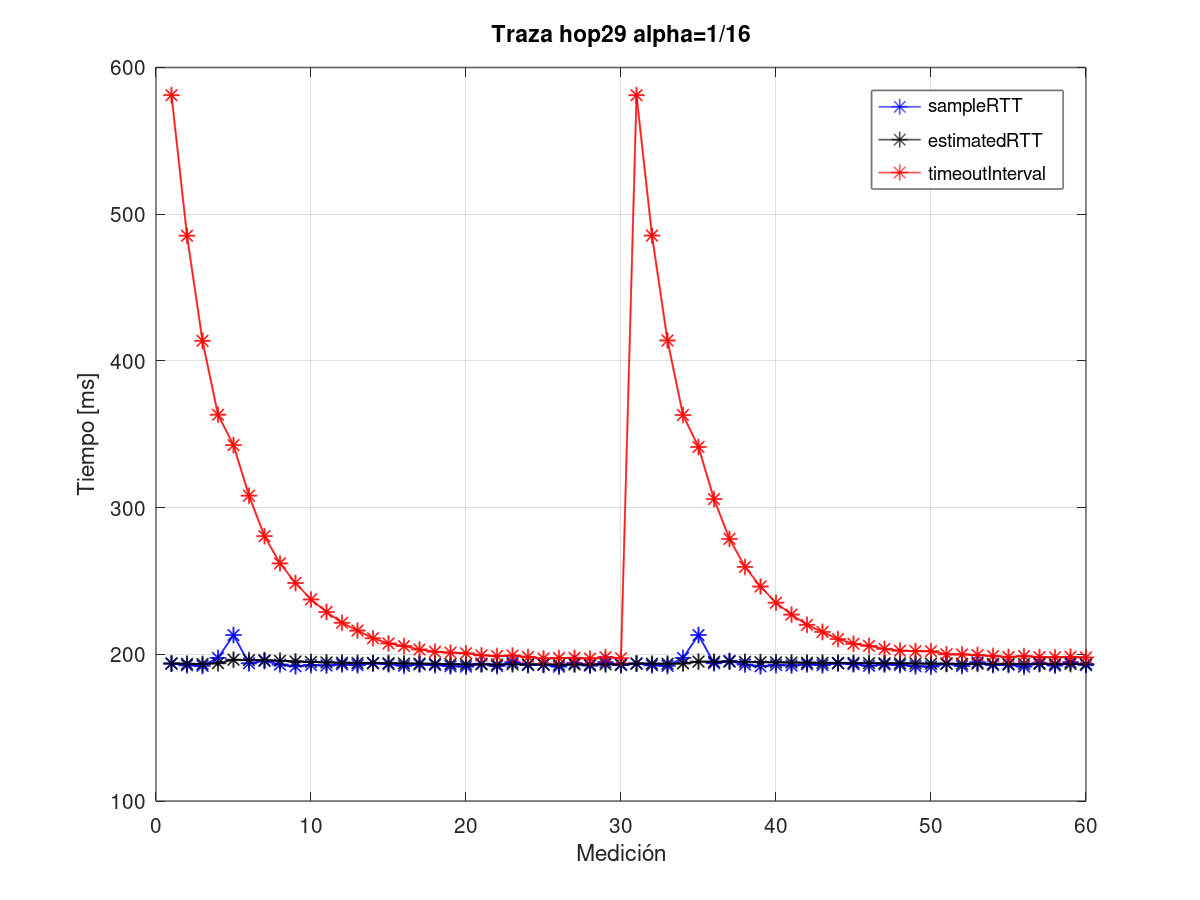
\includegraphics[width=0.75\textwidth]{img/alpha116/trazaHop29.png} 
  \caption{Gráfica de SampleRTT, EstimatedRTT y TimeoutInterval con \( \alpha = \frac{1}{16} \)
  de la muestra hop29}
  \label{fig:alpha2_p2}
\end{figure}

\subsection*{Discusión y Conclusiones}
\noindent A partir de las gráficas obtenidas y el análisis de los errores cuadráticos medios (ECM) 
para cada valor de \( \alpha \), podemos concluir que:

\begin{itemize}
    \item El valor de \( \alpha = \frac{1}{8} \) (por defecto) produce una estimación bastante precisa,
    con un ECM moderado.
    \item Un valor mayor de \( \alpha \), como \( \alpha_1 = \frac{1}{4} \), aumenta la sensibilidad
    del algoritmo, lo que puede generar un mayor error en entornos con fluctuaciones rápidas en
    \( \text{SampleRTT} \).
    \item Un valor menor de \( \alpha \), como \( \alpha_2 = \frac{1}{16} \), reduce la sensibilidad
    del algoritmo, lo que puede ser útil en entornos estables, pero puede no reaccionar rápidamente 
    ante cambios importantes en el RTT.
\end{itemize}



\end{document}